\subsection{Research Activities} \label{Research Activities section}
According to the exploratory experiment guidelines \cite{oivoSoftwareEngineeringResearch2004}, we apply different treatments to the same object.
We implement the process with an experiment of two phases:

\textbf{In the first phase, we reproduce the barren plateaus phenomenon.}
We use Qiskit \cite{Qiskit} to construct the ansatzes.
For each ansatz, we implement and apply four different methods (see Figure \ref{Research Activities Figure} and Table \ref{implementation of methods table}).
By definition of barren plateau as discussed in Section \ref{Literature Review section}, we would expect the shrinking rate of the variance values to be \textit{exponential} (see Figure \ref{Variance Shrinking demo}) if the initial parameter has landed in a barren plateau.
We keep track of the variance and the number of qubits to see if the variance is shrinking at this rate.
The result of the first phase is to determine which combinations of the ansatz and the BP treatment result in the shrinking rate of the loss function gradients.

\textbf{In the second phase, we implement the QNNs and measure their performances}.
With the ansatzes developed from the first step, we can implement the QNN models to test their performances.
The QNN models will be trained with standard data sets provided by Qiskit (refer to Section \ref{Resources section}).

The results of the research activities are discussed in the Subsection \ref{Data Collecting Section}.

\begin{table}[]
    \centering
    \begin{tabular}{|p{3cm}|p{2cm}|p{2cm}|p{2cm}|p{2cm}|}
        \hline
        \textbf{Method /\newline Aspect}      & \textbf{\#0:\newline No restrictions} & \textbf{\#1:\newline Local cost function, shallow circuits} & \textbf{\#2:\newline Identity Blocks} & \textbf{\#3:\newline Layerwise learning} \\
        \hline \hline
        \raggedright\emph{Ansatz depth}       & Any length                            & Bounded                                                     & Any length                            & Any length                               \\
        \hline
        \raggedright\emph{Cost Function}      & Global                                & Limited                                                     & All qubits                            & All qubits                               \\
        \hline
        \raggedright\emph{Initial Parameters} & Randomised                            & Randomised                                                  & Restricted                            & Restricted                               \\
        \hline
    \end{tabular}
    \caption{
        A comparison of different methods that applied to the ansatz in phase 1.
        The method $\#$0 is widely applied in construction of QNN ansatzes.
        The other three methods are discussed in Section \ref{Literature Review section}.
    }
    \label{implementation of methods table}
\end{table}


\begin{figure}
    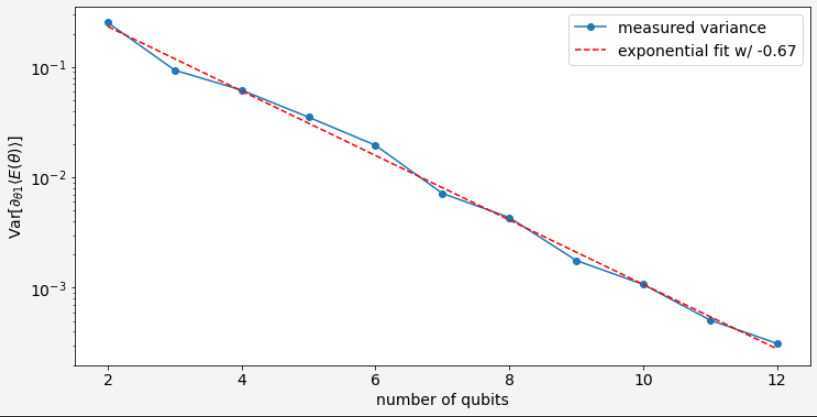
\includegraphics[width=\textwidth]{./ResearchDesign/Appendices/VarianceShrinking.png}
    \caption{
        An example of the barren plateaus phenomenon occurs in a QNN model.
        The variance of the gradient shrinks \textit{exponentially} with the number of qubits.
        Barren plateaus phenomenon prevents optimisation algorithms from navigating the cost function landscape efficiently.
    }
    \label{Variance Shrinking demo}
\end{figure}